\stepcounter{tableCounter} % Increment counter
\setcounter{rowCounter}{0} % Reset counter
\begin{tabularx}{\textwidth}{|>{\columncolor{tableColumnColor}}c|>{\columncolor{tableColumnColor}}c|>{\hsize=1.2\hsize}X|>{\hsize=.8\hsize}X|}
  \hline
  \rowcolor{tableHeaderColor}
  ID & Check & Description & Comments \\ \hline
  \multicolumn{4}{|c|}{\cellcolor{tableColumnColor} \textbf{Subsystem Preparation: } \textit{Can be performed one day prior to the test}} \\ \hline
  
  \cellcolor{cyan}
  \procedureItem{Write down starting time}{Start time:}
  
  \cellcolor{cyan}
  \procedureItem{If not immediately after briefing: 
    Gather everyone in front of the HANGAR and perform an attendance check (sec. B)}{}
  
  \cellcolor{cyan}
  \procedureItem{Show current phase on the \textit{Firing Organization Chart}}{}
  
  \cellcolor{cyan}
  \procedureItem{$\rightarrow$ TC informs about upcoming \textbf{Subsystem Preparation}}{}
  
  \cellcolor{cyan}
  \procedureItem{Hand out the following procedures:
    \begin{itemize}
      \item \textit{\underline{Assembly Engine}}
      \item \textit{\underline{Assembly Igniter}}
      \item \textit{\underline{Preparation PSS}}
      \item \textit{\underline{Preparation Control}}
      \item \textit{\underline{KiDAQ}}
    \end{itemize}
  }{}

  \multicolumn{4}{|c|}{\cellcolor{tableColumnColor} \textit{Work in Parallel}} \\ \hline
  
  \cellcolor{red}
  \procedureItem{Prepare ENGINE according to \textit{\underline{Assembly Engine, Assembly Igniter}}}{}
  
  \cellcolor{orange}
  \procedureItem{Prepare PSS according to \textit{\underline{Preparation PSS}}}{}
  
  \cellcolor{yellow}
  \procedureItem{If not already done: Install the Control station according to \textit{\underline{Installation Control}}}{}
  
  \cellcolor{yellow}
  \procedureItem{Prepare DACS according to \textit{\underline{Preparation Control}}}{}
  
  \cellcolor{yellow}
  \procedureItem{Prepare DACS according to \textit{\underline{KiDAQ}}}{}
  
  \cellcolor{cyan}
  \procedureItem{Collect completed and signed \textit{\underline{Assembly Engine}} from ENG1}{}
  
  \cellcolor{cyan}
  \procedureItem{Collect completed and signed \textit{\underline{Assembly Igniter}} from ENG1}{}
  
  \cellcolor{cyan}
  \procedureItem{Collect completed and signed \textit{\underline{Preparation PSS}} from PSS1}{}
  
  \cellcolor{cyan}
  \procedureItem{Collect completed and signed \textit{\underline{KiDAQ}}}{}
  
  \cellcolor{cyan}
  \procedureItem{Collect completed and signed \textit{\underline{Preparation Control}} from DACS1}{}
  
  \cellcolor{cyan}
  \procedureItem{$\rightarrow$ End of Subsystem Preparation}{}
  
  \multicolumn{4}{|c|}{\cellcolor{tableColumnColor} \textbf{Functionality Check \& Leakage Test: } \textit{Can be performed one day prior to the test}} \\ \hline
  
  \cellcolor{cyan}
  \procedureItem{Write down starting time}{Start Time:}
  
  \cellcolor{cyan}
  \procedureItem{Gather everyone in front of the HANGAR and perform an attendance check (sec. B)}{}
  
  \cellcolor{cyan}
  \procedureItem{$\rightarrow$ TC informs about upcoming \textbf{Functionality Check \& Leakage Test}}{}
  
  \cellcolor{cyan}
  \procedureItem{Only TC, SO, and PSS1/ENG1 are allowed to approach the trailer}{}
  
  \cellcolor{cyan}
  \procedureItem{Perform a Functionality Check Valves according to \textit{\underline{Functionality Check Valves}}}{}
  
  \cellcolor{cyan}
  \procedureItem{If the system has been disassembled/adapted since the last CF/FI:
    Perform a low-pressure leakage test of the system according to \textit{\underline{Low-Pressure Leakage Test PSS}}. 
    In parallel: DACS shall check sensor value and activation delays.
  }{Low-Pressure Leakage Tests can be performed in the Hangar}
  
  \multicolumn{4}{|c|}{\cellcolor{tableColumnColor} \textbf{Spark Plug Functionality Check: } \textit{Can be performed one day prior to the test}} \\ \hline

  \cellcolor{cyan}
  \procedureItem{Check that ENGINE compartment is cleared}{}
  
  \cellcolor{cyan}
  \procedureItem{Step back from the system ($>$ 2m). Nobody touching the trailer}{}
  
  \cellcolor{yellow}
  \procedureItem{$\leftrightarrow$ TC to DACS1: turn \textbf{IGNITION KEY} ON}{}
  
  \cellcolor{yellow}
  \procedureItem{$\leftrightarrow$ TC to DACS1: activate Spark Plug}{}
  
  \cellcolor{cyan}
  \procedureItem{Listen for spark}{}
  
  \cellcolor{yellow}
  \procedureItem{$\leftrightarrow$ TC to DACS1: deactivate Spark Plug}{}
  
  \cellcolor{yellow}
  \procedureItem{$\leftrightarrow$ TC to DACS1: turn \textbf{IGNITION KEY} OFF}{}
  
  \cellcolor{cyan}
  \procedureItem{If no spark:
    \begin{itemize}
      \item Check connections $\rightarrow$ go back to P-4.28
      \item If still no spark: Replace spark plug $\rightarrow$ go back to P-4.28
    \end{itemize}
  }{}
  
  \cellcolor{cyan}
  \procedureItem{$\rightarrow$ End of \textbf{FC \& Leakage Test}}{}
  
  \multicolumn{4}{|c|}{\cellcolor{tableColumnColor} \textbf{Packing: } \textit{Can be performed one day prior to the test}} \\ \hline

\cellcolor{cyan}
  \procedureItem{Write down starting time}{Start Time: }
  
  \cellcolor{cyan}
  \procedureItem{Gather everyone in front of the HANGAR and perform an attendance check (sec. B)}{}
  
  \cellcolor{cyan}
  \procedureItem{$\rightarrow$ TC informs about upcoming \textbf{Packing}}{}
  
  \cellcolor{cyan}
  \procedureItem{Hand out the following procedures:
    \begin{itemize}
      \item \textit{Material List}
    \end{itemize}
  }{}
  
  \multicolumn{4}{|c|}{\cellcolor{tableColumnColor} \textit{Work in Parallel}} \\ \hline

\cellcolor{green}
  \procedureItem{Pack safety equipment box according to \textit{\underline{Material List}}.
    Prepare cryo safety equipment for LOX Dewar Transport
  }{}
  
  \cellcolor{red}
  \procedureItem{Pack ENGINE box according to \textit{\underline{Material List}}}{}
  
  \cellcolor{orange}
  \procedureItem{Pack PSS box according to \textit{\underline{Material List}}}{}
  
  \cellcolor{yellow}
  \procedureItem{Pack DACS box according to \textit{\underline{Material List}}}{}
  
  \cellcolor{cyan}
  \procedureItem{Collect completed and signed \textit{\underline{Material List}} from SO}{}
  
  \cellcolor{cyan}
  \procedureItem{Collect completed and signed \textit{\underline{Material List}} from ENG1}{}
  
  \cellcolor{cyan}
  \procedureItem{Collect completed and signed \textit{\underline{Material List}} from PSS1}{}
  
  \cellcolor{cyan}
  \procedureItem{Collect completed and signed \textit{\underline{Material List}} from DACS1}{}
  
  \cellcolor{cyan}
  \procedureItem{$\rightarrow$ End of \textbf{Packing}}{}
  
  \multicolumn{4}{|c|}{\cellcolor{tableColumnColor} \textbf{Preparation for Transfer to Airfield: } \textit{To be performed on the day of firing}} \\ \hline

\cellcolor{cyan}
  \procedureItem{Write down starting time}{Start time: }
  
  \cellcolor{cyan}
  \procedureItem{Gather everyone in front of the HANGAR and perform an attendance check (sec. B)}{}
  
  \cellcolor{cyan}
  \procedureItem{$\rightarrow$ TC informs about upcoming \textbf{Preparation for Transfer}}{}

  \multicolumn{4}{|c|}{\cellcolor{tableColumnColor} \textit{Gas Bottle / Fuel Preparation}} \\ \hline
  
  \cellcolor{orange}
  \procedureItem{Get an N$_2$ Bottle (FSS PRZ) from the gas storage and place it on the trailer / in the car (only transport with open window)}{Bottle ID: }
  
  \cellcolor{orange}
  \procedureItem{Check that N$_2$ Bottle (FSS PRZ) is sufficiently full ($>$ 60 bar)}{}
  
  \cellcolor{orange}
  \procedureItem{Fix N$_2$ Bottle (FSS PRZ) onto the trailer / in the car using the attached belts and “Spanngurte” (for transport)}{}
  
  \cellcolor{orange}
  \procedureItem{Get an N$_2$ Bottle (OSS PRZ) from the gas storage and place it on the trailer / in the car (only transport with open window)}{Bottle ID: }
  
  \cellcolor{orange}
  \procedureItem{Check that N$_2$ Bottle (OSS PRZ) is sufficiently full ($>$ 130 bar)}{}
  
  \cellcolor{orange}
  \procedureItem{Fix N$_2$ Bottle (OSS PRZ) onto the trailer / in the car using the attached belts and “Spanngurte”}{}
  
  \cellcolor{orange}
  \procedureItem{Get an N$_2$ Bottle (PRG) from the gas storage and place it on the trailer / in the car (only transport with open window)}{Bottle ID: }
  
  \cellcolor{orange}
  \procedureItem{Check that N$_2$ Bottle (PRG) is sufficiently full ($>$ 100 bar)}{}
  
  \cellcolor{orange}
  \procedureItem{Fix N$_2$ Bottle (PRG) onto the trailer using the attached belts and “Spanngurte” (for transport). If no space on the trailer, use a car. Secure them properly in the car (Spanngurte). Never transport oxidizing and flammable gases/liquids in the same car (O$_2$ not in the same car as H$_2$ or Ethanol). Only transport with an open window}{}
  
  \cellcolor{orange}
  \procedureItem{Get H$_2$ Bottle from the gas storage. Check that H$_2$ Bottle is sufficiently full ($>$ \hl{TBD} bar). Load H$_2$ Bottle into the Emergency Car (keep the car's window open before loading into the car and during the transport)}{Bottle ID: }
  
  \cellcolor{orange}
  \procedureItem{Get the Ethanol Canisters from “Gefahrenstofflager” ($>$ \hl{TBD} L). Load Ethanol Canister into Emergency Car}{}
  
  \cellcolor{orange}
  \procedureItem{Get the O$_2$ Bottle from gas storage. Fix O$_2$ Bottle onto the trailer using the attached belts and “Spanngurte” (for transport) or put it in the car. Safety measures of -3.55 apply.}{}
  
  \cellcolor{orange}
  \procedureItem{\textit{LOX Dewar:}
    \begin{itemize}
      \item Wear safety goggles and cryo-gloves
      \item Get LOX Dewar from the LOX storage and place it in front of the HANGAR
      \item Ensure that pressure in the Dewar is more than 3 barg (check manometer on Dewar). If pressure is less than 3 barg, repressurize it by slowly opening the green knob. If SRVs open constantly, vent and repressurize on the airfield.
      \item Inspect wheels of Dewar before departure, they can be loose and break off.
    \end{itemize}
    $\rightarrow$ LOX Dewar is \textbf{ready for departure}
  }{Top view of the Dewar:
    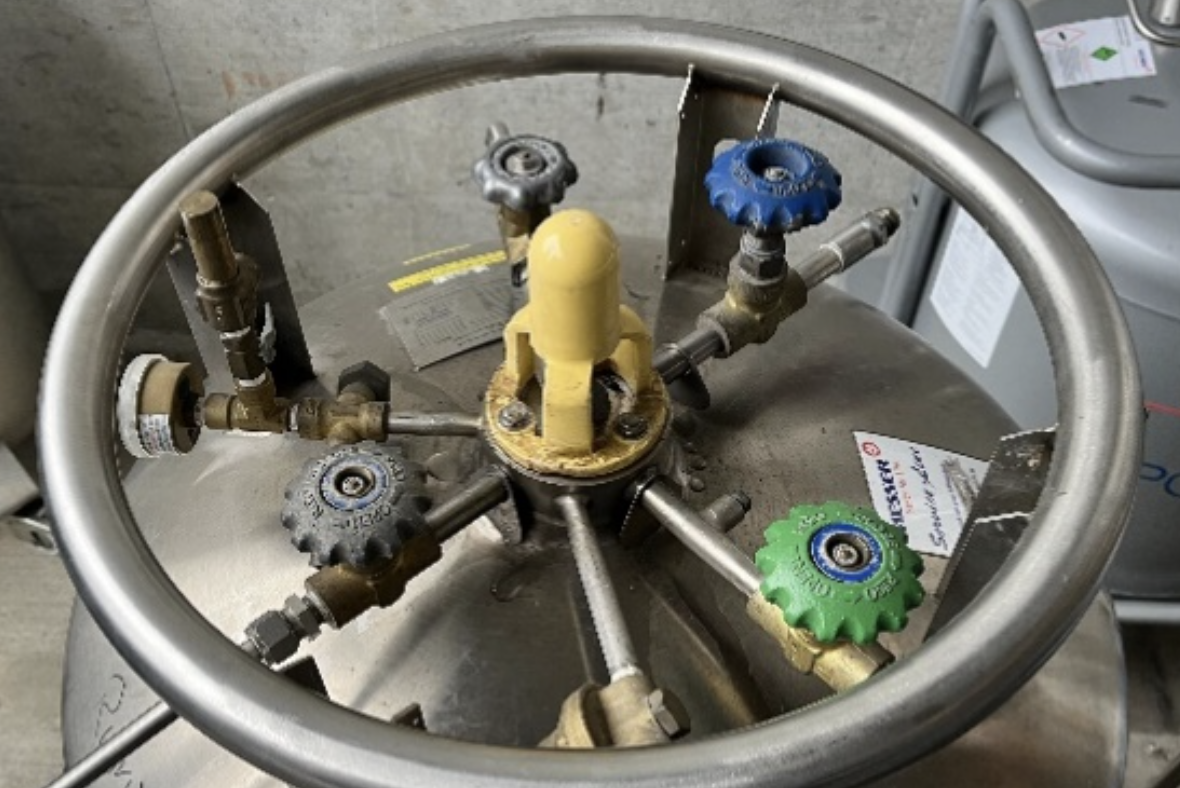
\includegraphics[width=\textwidth]{assets/picture-dewar.png}}
  
  \multicolumn{4}{|c|}{\cellcolor{tableColumnColor} \textit{Trailer, Water Pump, Dewar, Cable Roll \& Boxed Material Preparation}} \\ \hline

\cellcolor{red}
  \procedureItem{Prepare Trailer for Transport:
    \begin{itemize}
      \item Ensure there are no unfixed components on the trailer
      \item Fold up trailer side walls, fix them properly
      \item Fold down covers of the trailer, fix them properly
      \item Retract legs of the trailer
      \item Push trailer outside the HANGAR
      \item Attach trailer to towing vehicle (2nd Car)
    \end{itemize}
    $\rightarrow$ \textbf{Trailer} is ready for departure
  }{}
  
  \cellcolor{red}
  \procedureItem{Prepare Water Pump for Transport:
    \begin{itemize}
      \item Mount Water Pump on roller carriage (if not already done)
      \item Mount Water Container on roller carriage (if not already done)
      \item Push roller carriage outside the HANGAR
    \end{itemize}
    $\rightarrow$ \textbf{Water Pump} is ready for departure
  }{}
  
  \cellcolor{red}
  \procedureItem{Push Cable Roll outside the HANGAR
    $\rightarrow$ \textbf{Cable Roll} is ready for departure
  }{}
  
  \cellcolor{red}
  \procedureItem{Load boxed material into Cars (appropriate securing required):
    \begin{itemize}
      \item Emergency Car: GEN/SFTY/DACS/Snacks \& Beverages/Cable Roll
      \item 2nd Car: N$_2$ Bottles/Ethanol/H$_2$ Bottle/ENG/PSS/TOOL
    \end{itemize}
    $\rightarrow$ \textbf{Emergency Car} is ready for departure
  }{}
  
  \cellcolor{cyan}
  \procedureItem{$\rightarrow$ Ready for Transfer to Airfield}{}
  
\end{tabularx}